% Pipeline figure for Section~\ref{sec:method}: flow of the 731 tasks from
% SWE-Bench Pro v1.0 to the 642 released tasks.
% Band and bar heights are proportional to task counts (0.046 mm per task).
% Preamble: \usepackage{tikz,graphicx} (xcolor is loaded by tikz)
\definecolor{sbpFlag}{HTML}{4C72B0}
\definecolor{sbpRep}{HTML}{55A868}
\definecolor{sbpDisc}{HTML}{C44E52}
\definecolor{sbpKeep}{HTML}{7F7F7F}
\definecolor{sbpNone}{HTML}{B0B0B0}
\definecolor{sbpImg}{HTML}{8172B3}
\definecolor{sbpErr}{HTML}{DD8452}
\definecolor{sbpRes}{HTML}{64B5CD}
\begin{figure*}[t]
\centering
\resizebox{\textwidth}{!}{%
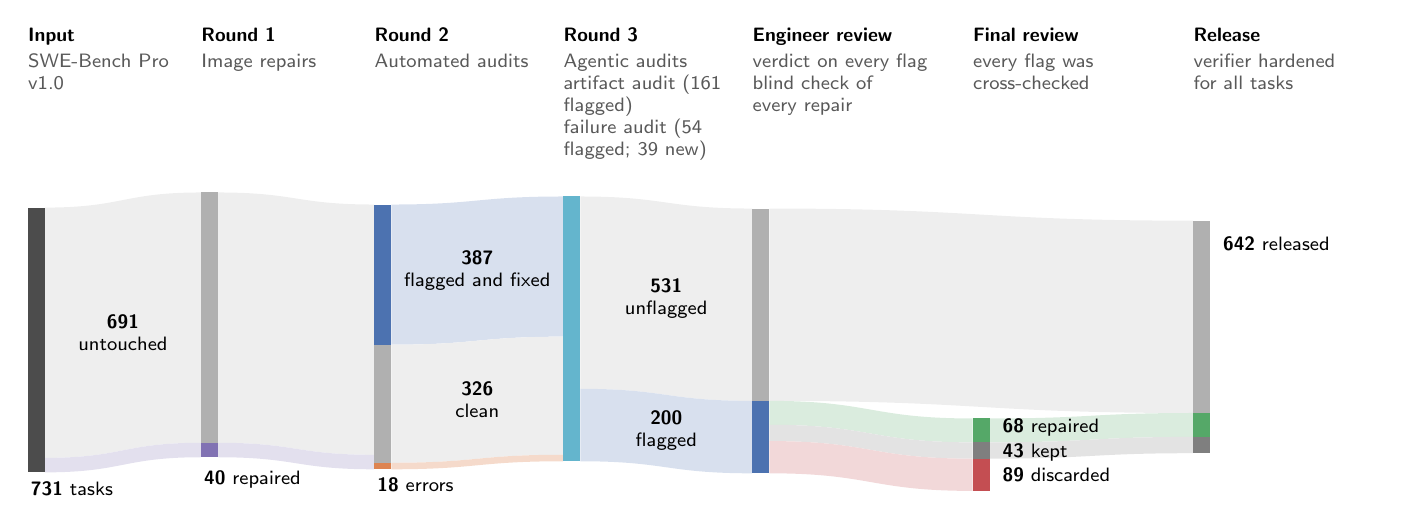
\begin{tikzpicture}[x=1mm, y=1mm, font=\sffamily\scriptsize,
  execute at begin node={\hyphenpenalty=10000\exhyphenpenalty=10000}]
% ---------------------------------------------------------------- bands
% Input -> Round 1: untouched / image repairs
\fill[sbpNone!22] (2.2,-1.92) .. controls (12.1,-1.92) and (12.1,0) .. (22,0)
  -- (22,-31.786) .. controls (12.1,-31.786) and (12.1,-33.706) .. (2.2,-33.706) -- cycle;
\fill[sbpImg!22] (2.2,-33.706) .. controls (12.1,-33.706) and (12.1,-31.786) .. (22,-31.786)
  -- (22,-33.626) .. controls (12.1,-33.626) and (12.1,-35.546) .. (2.2,-35.546) -- cycle;
% Round 1 -> Round 2
\fill[sbpNone!22] (24.2,0) .. controls (34.1,0) and (34.1,-1.53) .. (44,-1.53)
  -- (44,-33.316) .. controls (34.1,-33.316) and (34.1,-31.786) .. (24.2,-31.786) -- cycle;
\fill[sbpImg!22] (24.2,-31.786) .. controls (34.1,-31.786) and (34.1,-33.316) .. (44,-33.316)
  -- (44,-35.156) .. controls (34.1,-35.156) and (34.1,-33.626) .. (24.2,-33.626) -- cycle;
% Round 2 -> Result: flagged / clean / audit errors
\fill[sbpFlag!22] (46.2,-1.53) .. controls (57.1,-1.53) and (57.1,-0.51) .. (68,-0.51)
  -- (68,-18.312) .. controls (57.1,-18.312) and (57.1,-19.332) .. (46.2,-19.332) -- cycle;
\fill[sbpNone!22] (46.2,-19.332) .. controls (57.1,-19.332) and (57.1,-18.312) .. (68,-18.312)
  -- (68,-33.308) .. controls (57.1,-33.308) and (57.1,-34.328) .. (46.2,-34.328) -- cycle;
\fill[sbpErr!30] (46.2,-34.328) .. controls (57.1,-34.328) and (57.1,-33.308) .. (68,-33.308)
  -- (68,-34.136) .. controls (57.1,-34.136) and (57.1,-35.156) .. (46.2,-35.156) -- cycle;
% Result -> Round 3: unflagged / flagged
\fill[sbpNone!22] (70.2,-0.51) .. controls (81.1,-0.51) and (81.1,-2.04) .. (92,-2.04)
  -- (92,-26.466) .. controls (81.1,-26.466) and (81.1,-24.936) .. (70.2,-24.936) -- cycle;
\fill[sbpFlag!22] (70.2,-24.936) .. controls (81.1,-24.936) and (81.1,-26.466) .. (92,-26.466)
  -- (92,-35.666) .. controls (81.1,-35.666) and (81.1,-34.136) .. (70.2,-34.136) -- cycle;
% Round 3 -> Release: never flagged, bypasses engineer review
\fill[sbpNone!22] (94.2,-2.04) .. controls (121.1,-2.04) and (121.1,-3.58) .. (148,-3.58)
  -- (148,-28.006) .. controls (121.1,-28.006) and (121.1,-26.466) .. (94.2,-26.466) -- cycle;
% Round 3 -> Engineer review: repaired / kept / discarded
\fill[sbpRep!22] (94.2,-26.466) .. controls (107.1,-26.466) and (107.1,-28.7) .. (120,-28.7)
  -- (120,-31.736) .. controls (107.1,-31.736) and (107.1,-29.502) .. (94.2,-29.502) -- cycle;
\fill[sbpKeep!22] (94.2,-29.502) .. controls (107.1,-29.502) and (107.1,-31.736) .. (120,-31.736)
  -- (120,-33.806) .. controls (107.1,-33.806) and (107.1,-31.572) .. (94.2,-31.572) -- cycle;
\fill[sbpDisc!22] (94.2,-31.572) .. controls (107.1,-31.572) and (107.1,-33.806) .. (120,-33.806)
  -- (120,-37.9) .. controls (107.1,-37.9) and (107.1,-35.666) .. (94.2,-35.666) -- cycle;
% Engineer review -> Release
\fill[sbpRep!22] (122.2,-28.7) .. controls (135.1,-28.7) and (135.1,-28.006) .. (148,-28.006)
  -- (148,-31.042) .. controls (135.1,-31.042) and (135.1,-31.736) .. (122.2,-31.736) -- cycle;
\fill[sbpKeep!22] (122.2,-31.736) .. controls (135.1,-31.736) and (135.1,-31.042) .. (148,-31.042)
  -- (148,-33.112) .. controls (135.1,-33.112) and (135.1,-33.806) .. (122.2,-33.806) -- cycle;
% ---------------------------------------------------------------- nodes
\fill[black!70] (0,-35.546) rectangle (2.2,-1.92);
\fill[sbpNone]  (22,-31.786) rectangle (24.2,0);
\fill[sbpImg]   (22,-33.626) rectangle (24.2,-31.786);
\fill[sbpFlag]  (44,-19.332) rectangle (46.2,-1.53);
\fill[sbpNone]  (44,-34.328) rectangle (46.2,-19.332);
\fill[sbpErr]   (44,-35.156) rectangle (46.2,-34.328);
\fill[sbpRes]   (68,-34.136) rectangle (70.2,-0.51);
\fill[sbpNone]  (92,-26.466) rectangle (94.2,-2.04);
\fill[sbpFlag]  (92,-35.666) rectangle (94.2,-26.466);
\fill[sbpRep]   (120,-31.736) rectangle (122.2,-28.7);
\fill[sbpKeep]  (120,-33.806) rectangle (122.2,-31.736);
\fill[sbpDisc]  (120,-37.9) rectangle (122.2,-33.806);
\fill[sbpNone]  (148,-28.006) rectangle (150.2,-3.58);
\fill[sbpRep]   (148,-31.042) rectangle (150.2,-28.006);
\fill[sbpKeep]  (148,-33.112) rectangle (150.2,-31.042);
% ---------------------------------------------------------------- labels
\node[anchor=north west, inner sep=1pt] at (0,-36.3) {\textbf{731} tasks};
\node[align=center] at (12.1,-17.8) {\textbf{691}\\untouched};
\node[anchor=north west, inner sep=1pt] at (22,-35.0) {\textbf{40} repaired};
\node[align=center] at (57.1,-9.9) {\textbf{387}\\flagged and fixed};
\node[align=center] at (57.1,-26.3) {\textbf{326}\\clean};
\node[anchor=north west, inner sep=1pt] at (44,-35.8) {\textbf{18} errors};
\node[align=center] at (81.1,-13.5) {\textbf{531}\\unflagged};
\node[align=center] at (81.1,-30.3) {\textbf{200}\\flagged};
\node[anchor=west, inner sep=1pt] at (123.4,-29.9) {\textbf{68} repaired};
\node[anchor=west, inner sep=1pt] at (123.4,-33.0) {\textbf{43} kept};
\node[anchor=west, inner sep=1pt] at (123.4,-35.9) {\textbf{89} discarded};
\node[anchor=west, inner sep=1pt] at (151.4,-6.5) {\textbf{642} released};
% ---------------------------------------------------------------- stage headers
\node[anchor=north west, inner sep=0pt, text width=20mm, align=left] at (0,21)
  {{\bfseries Input}\\[1.5pt]\textcolor{black!65}{SWE-Bench Pro\\v1.0}};
\node[anchor=north west, inner sep=0pt, text width=20mm, align=left] at (22,21)
  {{\bfseries Round 1}\\[1.5pt]\textcolor{black!65}{Image repairs}};
\node[anchor=north west, inner sep=0pt, text width=22mm, align=left] at (44,21)
  {{\bfseries Round 2}\\[1.5pt]\textcolor{black!65}{Automated audits}};
\node[anchor=north west, inner sep=0pt, text width=22mm, align=left] at (68,21)
  {{\bfseries Round 3}\\[1.5pt]\textcolor{black!65}{Agentic audits\\artifact audit (161 flagged)\\failure audit (54 flagged; 39 new)}};
\node[anchor=north west, inner sep=0pt, text width=26mm, align=left] at (92,21)
  {{\bfseries Engineer review}\\[1.5pt]\textcolor{black!65}{verdict on every flag\\blind check of\\every repair}};
\node[anchor=north west, inner sep=0pt, text width=26mm, align=left] at (120,21)
  {{\bfseries Final review}\\[1.5pt]\textcolor{black!65}{every flag was\\cross-checked}};
\node[anchor=north west, inner sep=0pt, text width=24mm, align=left] at (148,21)
  {{\bfseries Release}\\[1.5pt]\textcolor{black!65}{verifier hardened\\for all tasks}};
\end{tikzpicture}}%
\caption{Flow of the 731 tasks from SWE-Bench Pro v1.0 to the released set;
bar and band heights are proportional to task counts. Round~1 repairs 40
container images (leaked test and fixture files, non-standard instructions).
Round~2's automated audit flags 387 tasks (all fixed by human experts). In Round~3, the artifact audit (an LLM agent and a human
auditor compare the instruction with the tests and reference patch) and the
failure audit (an LLM judge attributes failed runs of four agent setups) flag
200 tasks. Engineers adjudicate every flag, and a repair ships only after a
blind re-implementation of the edited instruction passes the hidden tests.}
\label{fig:pipeline}
\end{figure*}